\documentclass{../source/Experiment}

\major{信息工程}
\name{姚桂涛}
\title{降维技术}
\stuid{3190105597}
\college{信息与电子工程学院}
\date{\today}
\lab{教11-400}
\course{人工智能实验}
\instructor{胡浩基、魏准}
\grades{}
\expname{Principal Component Analysis}
\exptype{设计验证}
\partner{}
\begin{document}
    \makecover
    \section{实验题目}
        \subsection{实验4-1}
        利用PCA函数,对testSet.txt中数据做降维分析: (1)可视化topNfeat 分别等于1、2时,PCA的输出数据;(2)通过与原始数据对比,讨论topNfeat 分别等于1、2时的降维效果;


        \subsection{实验4-2}
       
        利用PCA,对secom.data数据降维,(1)讨论topNfeat 取值对降维数据的影响;(2)找到降维后恢复的数据与原始数据相对误差小于9\%的topNfeat
    
    \section{实验代码}
    \subsection{pca.py}
    \lstinputlisting[
        language  =   Python,
        title = {pca.py}
        ]{./Part4/pca.py}
    \subsection{实验4-1}
    \lstinputlisting[
            language  =   Python,
            title = {实验4-1}
        ]{./Part4/4_1.py}
    \subsection{实验4-2}
    \lstinputlisting[
            language  =   Python,
            title = {实验4-2}
        ]{./Part4/4_2.py}

    \section{实验结果}
        \subsection{实验4-1}
            topNfeat = 1:
            \begin{figure}[H]
                \centering
                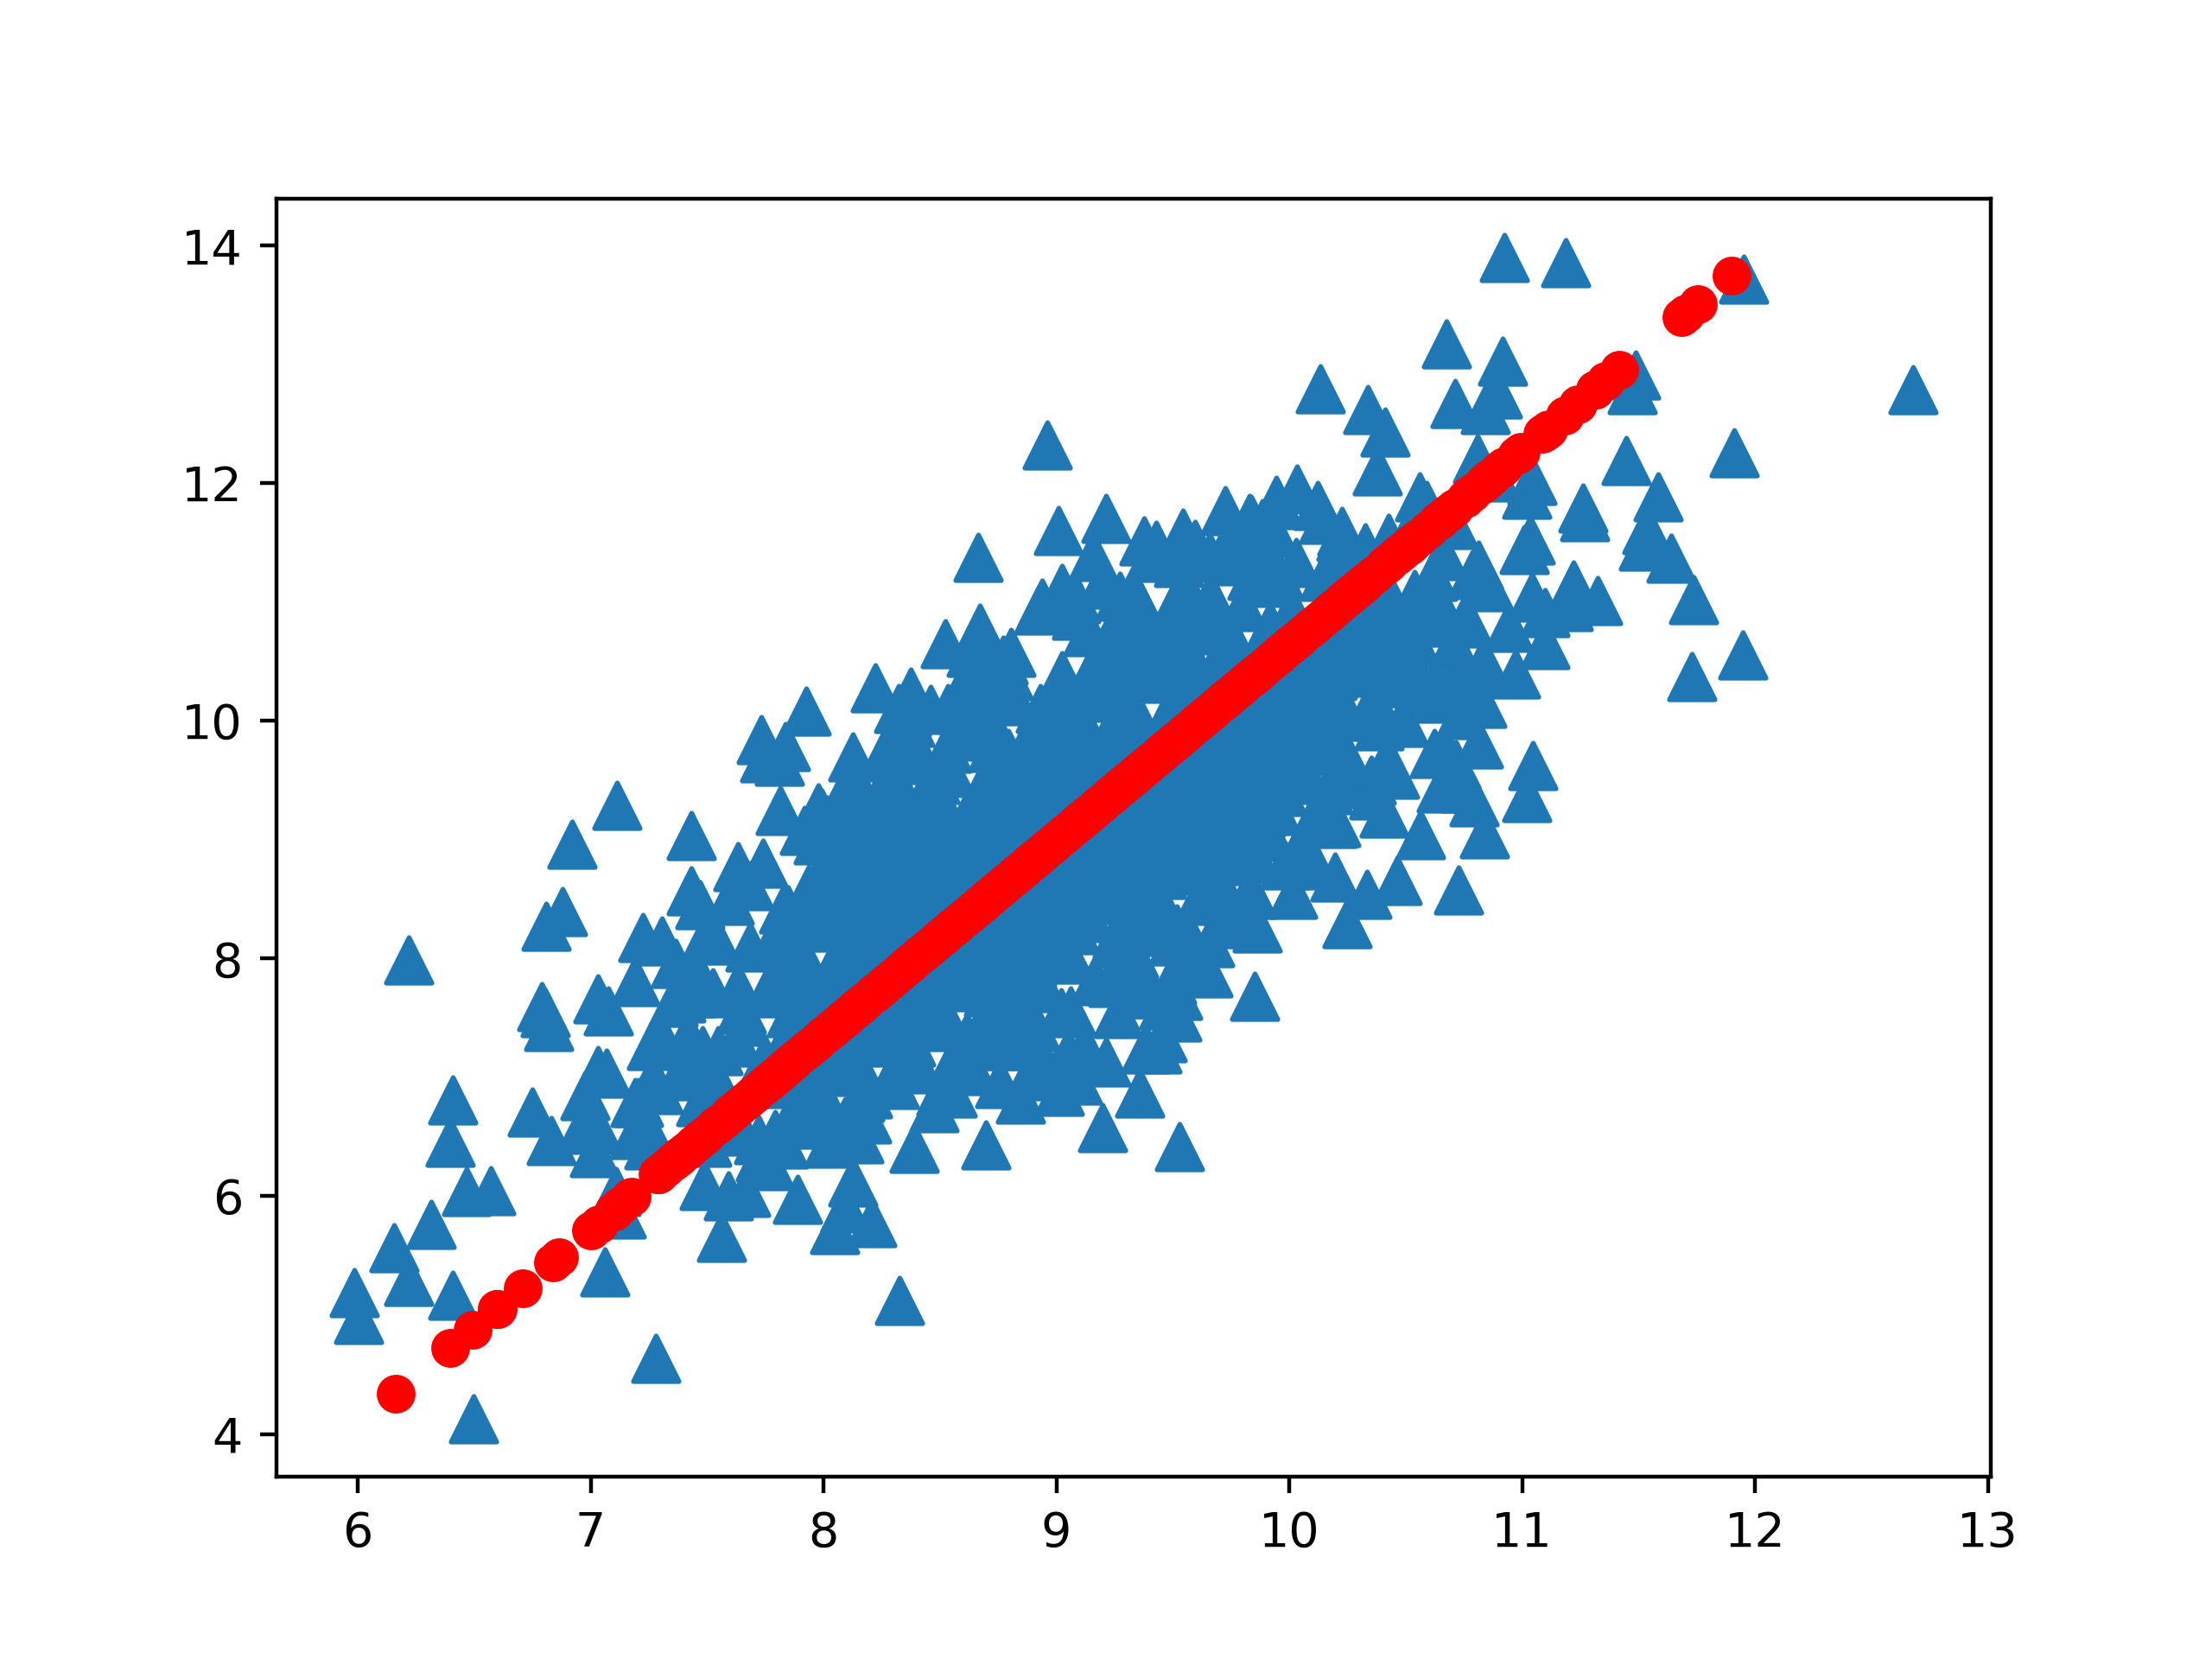
\includegraphics[width = 0.6\textwidth]{Part4/4-1-topNfeat(1).png}
                \caption{topNfeat = 1可视化}
            \end{figure}

            topNfeat = 2:
            \begin{figure}[H]
                \centering
                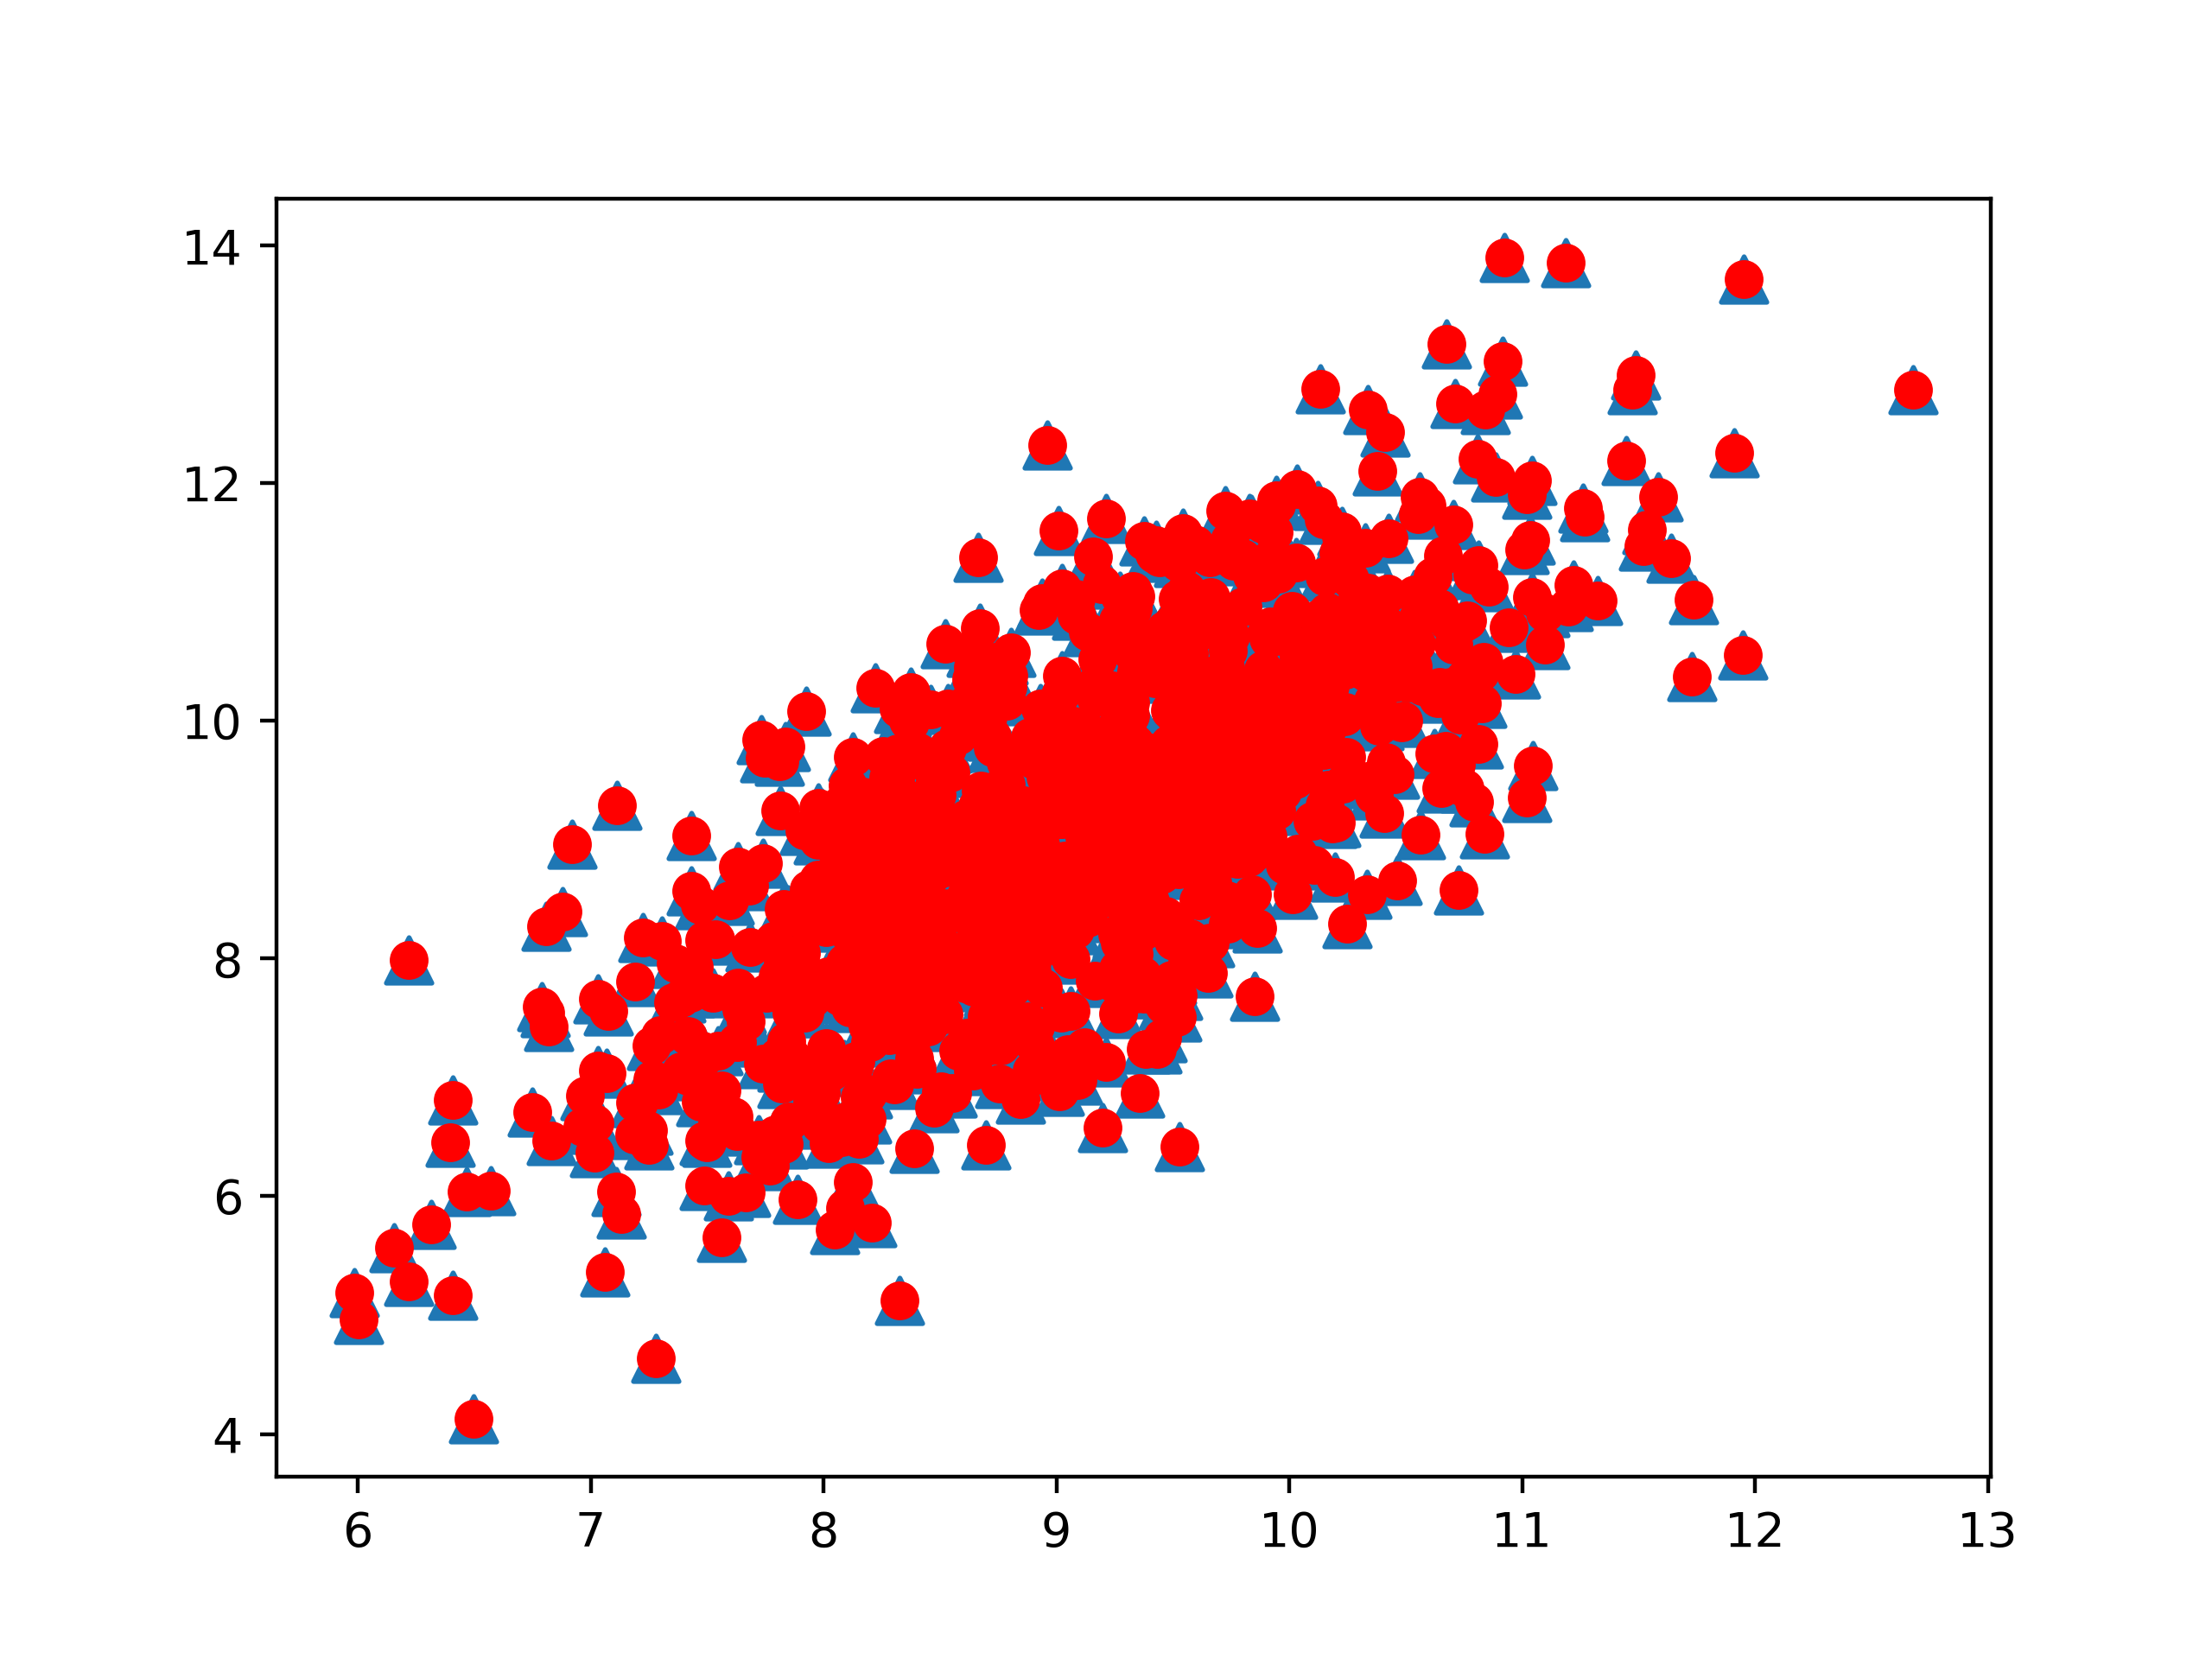
\includegraphics[width = 0.6\textwidth]{Part4/4-1-topNfeat(2).png}
                \caption{topNfeat = 2可视化}
            \end{figure}

            从可视化图可以看出,topNfeat = 1时,降维效果比较显著,而topNfeat = 2时,数据和原始数据重合,降维效果不好,这是因为原始数据只有两个特征,而topNfeat = 2并没有剔除任何特征。
            
    \subsection{实验4-2}
        topNfeat的取值影响了降维后数据与原始数据的误差,当topNfeat越小时,降维越大,但是误差也随之增大。

        经过实验找到降维后恢复的数据与原始数据相对误差小于9\%的topNfeat为8。
\end{document}


